% move all configuration stuff into one file so we can focus on the content
\documentclass[aspectratio=169,hyperref={pdfpagelabels=false,colorlinks=true,linkcolor=white,urlcolor=blue},t]{beamer}

%%%%%%%%%%%%%%%%%%%%%%%%%%%%%%%%%%%%%%%%%%%%%%%%%%%%%%%%%%%%%%%%%%%%%%%%%%%%%%%%%%
%%%%%%%%%%%%%%%%%%%%%%%%%%%%%%%%%%%%%%%%%%%%%%%%%%%%%%%%%%%%%%%%%%%%%%%%%%%%%%%%%%
% packages
\usepackage{pict2e}
\usepackage{epic}
\usepackage{amsmath,amsfonts,amssymb}
\usepackage{units}
\usepackage{fancybox}
\usepackage[absolute,overlay]{textpos} 
\usepackage{media9} % avi2flv: "C:\Program Files\ffmpeg\bin\ffmpeg.exe" -i TuneFreqFilterbank.avi -b 600k -s 441x324 -r 15 -acodec copy TuneFreqFilterbank.flv
\usepackage{animate}
\usepackage{gensymb}
\usepackage{multirow}
\usepackage{silence}
\usepackage[backend=bibtex,style=ieee]{biblatex}
\AtEveryCitekey{\iffootnote{\tiny}{}}
\addbibresource{references}

%%%%%%%%%%%%%%%%%%%%%%%%%%%%%%%%%%%%%%%%%%%%%%%%%%%%%%%%%%%%%%%%%%%%%%%%%%%%%%%%%%
%%%%%%%%%%%%%%%%%%%%%%%%%%%%%%%%%%%%%%%%%%%%%%%%%%%%%%%%%%%%%%%%%%%%%%%%%%%%%%%%%%
% relative paths
\graphicspath{{graph/}}


%%%%%%%%%%%%%%%%%%%%%%%%%%%%%%%%%%%%%%%%%%%%%%%%%%%%%%%%%%%%%%%%%%%%%%%%%%%%%%%%%%
%%%%%%%%%%%%%%%%%%%%%%%%%%%%%%%%%%%%%%%%%%%%%%%%%%%%%%%%%%%%%%%%%%%%%%%%%%%%%%%%%%
% units
\setlength{\unitlength}{1mm}

%%%%%%%%%%%%%%%%%%%%%%%%%%%%%%%%%%%%%%%%%%%%%%%%%%%%%%%%%%%%%%%%%%%%%%%%%%%%%%%%%%
%%%%%%%%%%%%%%%%%%%%%%%%%%%%%%%%%%%%%%%%%%%%%%%%%%%%%%%%%%%%%%%%%%%%%%%%%%%%%%%%%%
% theme & layout
\usetheme{Frankfurt}
\beamertemplatenavigationsymbolsempty
%\setbeamertemplate{frametitle}[smoothbars theme]
\setbeamertemplate{frametitle}
{
    \begin{beamercolorbox}[ht=1.8em,wd=\paperwidth]{frametitle}
        \vspace{-.1em}%
        \hspace{.2em}{\strut\insertframetitle\strut}
        
        \hspace{.2em}\small\strut\insertframesubtitle\strut
        %\hfill
        %
\includegraphics[height=.8cm,keepaspectratio]{CenterMusicTechnology-solid-2lines-white-CoAtag}
        
    \end{beamercolorbox}
    \begin{textblock*}{100mm}(11.6cm,.7cm)
        \includegraphics[height=.8cm,keepaspectratio]{logo_GTCMT_black}
    \end{textblock*}
}

% set this to ensure bulletpoints without subsections
\usepackage{remreset}
\makeatletter
\@removefromreset{subsection}{section}
\makeatother
\setcounter{subsection}{1}

%---------------------------------------------------------------------------------
% appearance
\setbeamercolor{structure}{fg=gtgold}
\setbeamercovered{transparent} %invisible
\setbeamercolor{bibliography entry author}{fg=black}
\setbeamercolor*{bibliography entry title}{fg=black}
\setbeamercolor*{bibliography entry note}{fg=black}

%\usepackage{pgfpages}
%\setbeameroption{show notes}
%\setbeameroption{show notes on second screen=right}
%---------------------------------------------------------------------------------
% fontsize
\let\Tiny=\tiny

%%%%%%%%%%%%%%%%%%%%%%%%%%%%%%%%%%%%%%%%%%%%%%%%%%%%%%%%%%%%%%%%%%%%%%%%%%%%%%%%%%
%%%%%%%%%%%%%%%%%%%%%%%%%%%%%%%%%%%%%%%%%%%%%%%%%%%%%%%%%%%%%%%%%%%%%%%%%%%%%%%%%%
% warnings
\pdfsuppresswarningpagegroup=1
\WarningFilter{biblatex}{Patching footnotes failed}
\WarningFilter{latexfont}{Font shape}
\WarningFilter{latexfont}{Some font shapes}
\WarningFilter{gensymb}{Not defining}



\subtitle{Part 3.1: Fundamentals I}

%%%%%%%%%%%%%%%%%%%%%%%%%%%%%%%%%%%%%%%%%%%%%%%%%%%%%%%%%%%%%%%%%%%%%%%%%%%%
\begin{document}
    % generate title page
	

\begin{frame}
    \titlepage
    %\vspace{-5mm}
    \begin{flushright}
        \href{http://www.gtcmt.gatech.edu}{\includegraphics[height=.8cm,keepaspectratio]{logo_GTCMT_black}}
    \end{flushright}
\end{frame}


    \section[overview]{lecture overview}
        \begin{frame}{introduction}{overview}
            \begin{itemize}
                \item   \textbf{text book}  
                    \begin{itemize}
                        \item   \href{http://ieeexplore.ieee.org/xpl/ebooks/bookPdfWithBanner.jsp?fileName=6331119.pdf&bkn=6266785&pdfType=chapter}{\underline{\textit{Chapter 2: Fundamentals} (pp.~7--17)}}
                    \end{itemize}
                \item   \textbf{additional reading}  
                    \begin{itemize}
                        \item   Richard G.~Lyons, \textit{Understanding Digital Signal Processing}, 3rd, Prentice Hall/Pearson, 2011
                    \end{itemize}
                \bigskip
                \item<2->   \textbf{lecture content}
                    \begin{itemize}
                        \item<2->   periodic and random signals
                        \item<3->   sampling and quantization
                        \item<4->   statistical signal description
                        \item<5->   convolution
                    \end{itemize}
            \end{itemize}
        \end{frame}
        
    \section[intro]{introduction}
        \begin{frame}{audio signals}{signal categories}
            \begin{itemize}
                \item	\textbf{deterministic signals}:\\
                        \textit{predictable}: future shape of the signal can be known (example: sinusoidal)
                \pause		
                \item	\textbf{random signals}:\\
                        \textit{unpredictable}: no knowledge can help to predict what is coming next (example: white noise)
            \end{itemize}
            
            \bigskip
            \pause
            ``real-world'' audio signals can be modeled as time-variant combination of 
            \begin{itemize}
                \item	(quasi-)periodic parts
                \item	(quasi-)random parts
            \end{itemize}
        \end{frame}

    \section[signals]{signals}
        \begin{frame}{audio signals}{periodic signals 1/5}
            \setbeamercovered{invisible}

            periodic signals: most prominent examples of deterministic signals
            \begin{eqnarray*}
                x(t) 	&=& x(t+T_0)\\
                f_0 	&=& \frac{1}{T_0} =  \frac{\omega_0}{2\pi}
            \end{eqnarray*}

            \only<2>{
                \figwithmatlab{PeriodicRandom}
             }
            \vphantom{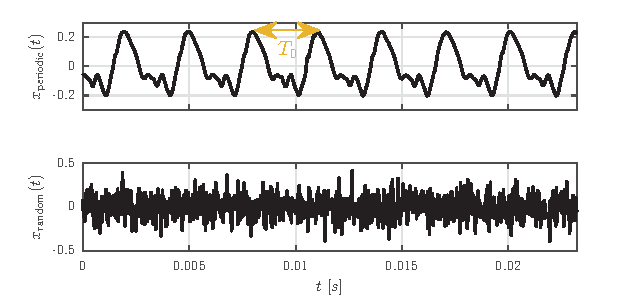
\includegraphics{PeriodicRandom}}
        \end{frame}

        \begin{frame}{audio signals}{periodic signals 2/5}
            periodic signal $\Rightarrow$ representation in \textbf{Fourier series}\footnote{\tiny Jean-Baptiste Joseph Fourier, 1768--1830}
            \begin {equation*}
                x(t) = \sum\limits_{k=-\infty}^{\infty} {\color<5>{gtgold}{a_k}} {\color<4>{gtgold}{\e^{\mathrm{j}{\color<2-3>{gtgold}{\omega_0}} {\color<3>{gtgold}{k}} t}}} \nonumber
            \end {equation*}
            \begin{itemize}
                \item<2-> $\omega_0 = 2\pi\cdot f_0$
                \item<3-> $k\omega_0$: integer multiples of the lowest frequency
                \item<4-> $\e^{\jom_0kt} = \cos(\omega_0kt) + \mathrm{j} \sin(\omega_0kt)$
                \item<5-> $a_k$: Fourier coefficients --- amplitude of each component
                    \begin {equation*}\label{eq:fourier_coeff}
                        a_k = \frac{1}{T_0}\int\limits_{-\nicefrac{T_0}{2}}^{\nicefrac{T_0}{2}} x(t) \e^{-\jom_0kt}\, dt \nonumber
                    \end {equation*}
            \end{itemize}
        \end{frame}

        \begin{frame}{audio signals}{periodic signals 3/5}
            \toremember{}
            
            \begin{block}{Fourier series}
                \begin{itemize}
                    \item   \textbf{every} periodic signal can be represented in a Fourier series
                    \item   a periodic signal \textbf{contains only} frequencies at integer multiples of the fundamental frequency $f_0$
                    \bigskip
                    \item<2->   Fourier series can only be applied to periodic signals
                    \item<2->   Fourier series is analytically elegant but only of limited practical use as the fundamental period has to be known
                \end{itemize}
            \end{block}
        \end{frame}

        \begin{frame}{audio signals}{periodic signals 4/5}
            reconstruction of periodic signals with limited number of sinusoidals:
            \begin {equation*}
                \hat{x}(t) = \sum\limits_{k=-\mathcal{K}}^{\mathcal{K}} a_k e^{\jom_0kt}
            \end {equation*}
            %\vspace{-5mm}
            \only<1>{
                \figwithref{AdditiveSynthesisSaw-1}%{matlab/displayAdditiveSynthesis.m}
            }
            
            \setcounter{i}{1}
            \whiledo{\value{i}<6}	
            {
                \pause
                \only<\value{beamerpauses}>
                {
                    \begin{figure}
                        \centering
                        \includegraphics{graph/AdditiveSynthesisSaw-\arabic{i}}
                    \end{figure}
                    \audioautoplay{additivesynthesis_saw_\arabic{i}}
                    
                    \addreference{matlab source: matlab/displayAdditiveSynthesis.m}
                }
                \stepcounter{i} 
            }	
            
            \setcounter{i}{1}
            \whiledo{\value{i}<6}	
            {
                \pause
                \only<\value{beamerpauses}>
                {
                    \begin{figure}
                        \centering
                        \includegraphics{graph/AdditiveSynthesisRect-\arabic{i}.pdf}
                    \end{figure}
                    \audioautoplay{additivesynthesis_rect_\arabic{i}}
                    
                    \addreference{matlab source: matlab/displayAdditiveSynthesis.m}
                }
                \stepcounter{i} 
            }	
        \end{frame}
        \begin{frame}{audio signals}{periodic signals 5/5}
            youtube example --- mechanical additive synthesis:
            
            \url{http://youtu.be/8KmVDxkia_w}
        \end{frame}

        \begin{frame}{audio signals}{random process 1/2}
            \textbf{random process}: ensemble of random series
            \figwithmatlab{RandomProcess}%{matlab/displayRandomProcess.m}
        \end{frame}

        \begin{frame}{audio signals}{random process 2/2}
            \toremember{}
            
            \begin{block}{random process}
                \begin{itemize}
                    \item   ensemble of random series
                    \item   each series represents a \textit{sample} or the process
                    \item   the value of the next sample is indetermined, regardless of any amount of knowledge
                \end{itemize}
            \end{block}
            \begin{itemize}
                \item   special case: \textbf{stationarity}\\ all properties (such as the mean) are time invariant
                \item   example: white noise
            \end{itemize}
        \end{frame}

        \begin{frame}{audio signals}{matlab exercise}
            \matlabexercise{signal generation and plotting}
            
            \begin{enumerate}
                \item   generate a sinusoidal
                    \begin{itemize}
                        \item   4 periods
                        \item   max amplitude $0.707$
                    \end{itemize}
                \item   plot the sinusoidal
                \item   generate white noise 
                    \begin{itemize}
                        \item   uniform distribution
                        \item   approx. zero mean
                        \item   max amplitude $0.707$
                    \end{itemize}
                \item   plot the noise
            \end{enumerate}
        \end{frame}
            
    \section[digital signals]{digital signals}
        \begin{frame}{digital signals}{introduction}
            \textit{digital} signals are represented with a limited number of values
            \pause
            
            \bigskip
            $\Rightarrow$
            \begin{enumerate}
                \item	\textbf{sampling}: time discretization
                
                continuous time $\mapsto$ discrete equidistant points in time 
                
                
                \smallskip
                \item	\textbf{quantization}: amplitude discretization
                
                continuous amplitude $\mapsto$ discrete, pre-defined, set of values
            \end{enumerate}
        \end{frame}
        
        \subsection{sampling}
        \begin{frame}{digital signals}{sampling}
            \figwithref{Sampling01}
                
            \begin{itemize}
                \item   $f_\mathrm{S}\;[\unit{Hz}]$: number of samples per second
                \item   $T_\mathrm{S} = \nicefrac{1}{f_\mathrm{S}}\;[\unit{s}]$: distance between two neighboring samples
            \end{itemize}
        \end{frame}
            
        \begin{frame}{digital signals}{sampling frequencies}
            \question{What are typical sample rates}
            
            
            \begin{itemize}
                \item	\unit[8--16]{kHz}: speech (phone)
                \item	\unit[44.1--48]{kHz}: (consumer) audio/music
                \item	\unit[$>$48]{kHz}: production audio
            \end{itemize}
            \pause
            
            \bigskip
            \begin{table}
                \centering
                    \begin{tabular}{l|cccccc}
                        $f_\mathrm{S}$ & \unit[44.1]{kHz} & \unit[32]{kHz} & \unit[22.05]{kHz} & \unit[16]{kHz} & \unit[8]{kHz} & \unit[6]{kHz}\\
                        & \includeaudio{sampling_44}& \includeaudio{sampling_32}& \includeaudio{sampling_22}& \includeaudio{sampling_16}& \includeaudio{sampling_08}& \includeaudio{sampling_06} \\
                    \end{tabular}
            \end{table}
        \end{frame}	
            
        \begin{frame}{digital signals}{sampling ambiguity}
            \figwithmatlab{Sampling02}
        \end{frame}	
        
        \begin{frame}{digital signals}{sampling ambiguity --- wagon-wheel effect}
            \only<1>{\figwithref{StageCoach}{\url{flickr.com/photos/fotoguy49057/12209056184}}}
            \visible<2->{
                compare speed of wheel (spokes) $f_\mathrm{wheel}$ between real world and video recording for an accelerating stage coach
                \begin{columns}
                    \column{0.5\textwidth}
                        
                        \begin{enumerate}
                            \item<2->	$f_\mathrm{wheel} < \frac{f_\mathrm{S}}{2}$\\
                                speeding up
                            \item<3->	$\frac{f_\mathrm{S}}{2} < f_\mathrm{wheel} < f_\mathrm{S}$\\
                                slowing down
                            \item<4->	$f_\mathrm{wheel} = f_\mathrm{S}$:\\
                            standing still
                            \item<4->	$\ldots$
                        \end{enumerate}
                                    
                    \column{0.5\textwidth}
                        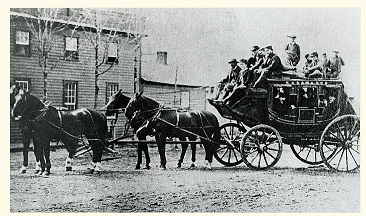
\includegraphics[scale=0.5]{StageCoach}
                \end{columns}
            }
            
            \only<5->{
            \vspace{5mm}
            video example: \url{https://youtu.be/QYYK4tlCMlY}
            }
        \end{frame}	
        
        \begin{frame}{digital signals}{sampling ambiguity --- spectral domain}
            \videowithmatlab{animateSampling}
            \question{What are the x-axis labels for the spectrum shown above?}
        \end{frame}	
        
        \begin{frame}{digital signals}{sampling theorem}
            \toremember{}
            
            \begin{block}{sampling theorem}
                A sampled signal can be reconstructed without loss of information if the sample rate $f_\mathrm{S}$ is higher than twice the bandwidth $f_\mathrm{max}$ of the original audio signal.
                
                \begin{equation*}
                    f_\mathrm{S} > 2\cdot f_\mathrm{max}
                \end{equation*}
            \end{block}
            
            \pause
            \bigskip
            $\nicefrac{f_\mathrm{S}}{2}$ is sometimes referred to as the \textit{Nyquist}\footnote{\tiny Harry Nyquist, 1889--1976}-rate
        \end{frame}	

        \begin{frame}{digital signals}{matlab exercise}
            \matlabexercise{sampling}
            
            \begin{enumerate}
                \item   generate a sinesweep
                    \begin{itemize}
                        \item   length: \unit[5]{s}
                        \item   1000--20000\unit{Hz}
                        \item   sample rate: \unit[48000]{Hz}
                        \item   max amplitude: $0.5$
                    \end{itemize}
                \item   generate a new signal by taking only every 4th sample
                \item   listen to and compare both signals
            \end{enumerate}
        \end{frame}
            

        \subsection{quantization}
        \begin{frame}{digital signals}{quantization}
        
            \begin{itemize}
                \item   map continuous amplitude values to pre-defined set of values
                \item<2->   quantization steps are most frequently \textbf{equidistant}
                \item<2->   signal stored in binary $\Rightarrow$ \# quantization steps \textbf{power of 2}
                \item<3->   \textbf{example: 4-bit quantization}
                    \begin{itemize}
                        \item	\textit{number of quantization steps}: $\mathcal{M} = 16$
                        \item	\textit{word length}: $w = \log_2(\mathcal{M}) = \unit[4]{bit}$
                    \end{itemize}
            \end{itemize}
            
            \vspace{-3mm}
            \visible<3->{
            \figwithmatlab{Quantization}}
        \end{frame}	

        \begin{frame}{digital signals}{quantization wordlength}
            \question{What are typical wordlengths?}
            
            \begin{itemize}
                \item	\unit[8]{bit}: speech
                \item	\unit[12--14]{bit}: low quality audio
                \item	\unit[16]{bit}: (consumer) audio/music
                \item	\unit[$>$16]{bit}: production audio
            \end{itemize}
            \pause
            
            \bigskip
            \begin{table}
                \centering
                    \begin{tabular}{l|ccccc}
                        $w$ & \unit[16]{bit} & \unit[12]{bit} & \unit[8]{bit} & \unit[4]{bit} &\unit[2]{bit}\\
                        & \includeaudio{quantized_16}& \includeaudio{quantized_12}& \includeaudio{quantized_8}& \includeaudio{quantized_4}& \includeaudio{quantized_2} \\
                    \end{tabular}
            \end{table}
        \end{frame}	

        \begin{frame}{digital signals}{quantization error}
            \begin{figure}
                \begin{footnotesize}
				\begin{picture}(90,15)
					\setcounter{iXOffset}{0}
					\setcounter{iYOffset}{0}
					\setcounter{iXBlockSize}{10}
					\setcounter{iYBlockSize}{10}
					\setcounter{iYBlockSizeDiv2}{5}
					\setcounter{iDistance}{5}
	
					\addtocounter{iYOffset}{\value{iYBlockSizeDiv2}}
	
					\put(\value{iXOffset}, \value{iYOffset})
						{\text{$x(i)$}}
					\addtocounter{iXOffset}{1}
	
					\addtocounter{iXOffset}{\value{iDistance}}
	
					\put(\value{iXOffset}, \value{iYOffset})
						{\vector(1,0){\value{iDistance}}}
	
					\addtocounter{iXOffset}{\value{iDistance}}
					\addtocounter{iYOffset}{-\value{iYBlockSizeDiv2}}
					
					\put(\value{iXOffset}, \value{iYOffset})
						{\framebox(\value{iXBlockSize}, \value{iYBlockSize}) {Q}}
	
					\addtocounter{iXOffset}{\value{iXBlockSize}}
					\addtocounter{iYOffset}{\value{iYBlockSizeDiv2}}
	
					\put(\value{iXOffset}, \value{iYOffset})
						{\vector(1,0){\value{iDistance}}}
	
					\addtocounter{iXOffset}{\value{iDistance}}
					\addtocounter{iXOffset}{1}

					\put(\value{iXOffset}, \value{iYOffset})
						{\text{$x_\mathrm{Q}(i)$}}


					\setcounter{iYOffset}{0}
					\addtocounter{iXOffset}{20}
					\addtocounter{iYOffset}{\value{iYBlockSizeDiv2}}
	
					\put(\value{iXOffset}, \value{iYOffset})
						{\text{$x(i)$}}
					\addtocounter{iXOffset}{1}
	
					\addtocounter{iXOffset}{\value{iDistance}}
					\put(\value{iXOffset}, \value{iYOffset})
						{\vector(1,0){\value{iDistance}}}

                    \put(57.3, 4.2)
                        {$\oplus$}

					\put(58.5, 10.6)
						{\vector(0,-1){\value{iDistance}}}

					\put(59, 11)
						{\text{$q(i)$}}
					
                    \addtocounter{iXOffset}{\value{iDistance}}
                    \addtocounter{iXOffset}{1}
					\put(\value{iXOffset}, \value{iYOffset})
						{\vector(1,0){\value{iDistance}}}

					\addtocounter{iXOffset}{\value{iDistance}}
					\addtocounter{iXOffset}{1}

					\put(\value{iXOffset}, \value{iYOffset})
						{\text{$x_\mathrm{Q}(i) = x(i) + q(i)$}}
				\end{picture}
\end{footnotesize}

            \end{figure}
            \bigskip
            \pause
            
            model for quantization: quantization noise $q$ is added to input signal $x$
            \begin{equation*}
                q(i) = x(i) - x_{\mathrm{Q}}(i)
            \end{equation*}
        \end{frame}		
        \begin{frame}{digital signals}{quantization error size}
            \question{What is the maximum amplitude of the quantization error?}

            \figwithmatlab{QuantizationError}
        \end{frame}	

        \begin{frame}{digital signals}{quantization error properties}
            Under the assumption that the signal has a variance much higher than the quantization step size, we find that the quantization error
            \begin{itemize}
                \item   is white noise and uncorrelated to signal,
                \item   is uniformly distributed, and
                \item   its power $W_\mathrm{Q}$ is directly related to the wordlength.
            \end{itemize}
            
            \pause
            \bigskip
            The quantizer quality is usually given by its \textit{Signal-to-Noise Ratio (SNR)}
			\begin{equation*}\label{eq:snr}
				SNR = 10\cdot\log_{10}\left(\frac{W_{\mathrm{S}}}{W_{\mathrm{Q}}}\right)\; [dB] 
			\end{equation*}
            
            \end{frame}	
            
            \begin{frame}{digital signals}{quantization: SNR}
                \toremember{}
                \begin{block}{signal-to-noise ratio (quantizer)}
                    \centering
                    \begin{equation*}
                        SNR = 6.02\cdot w + c_{\mathrm{S}}\quad [dB]
                    \end{equation*}
                    \vspace{-3mm}
                    \begin{itemize}
                        \item	every additional bit adds app.\ \unit[6]{dB} SNR
                        \item	constant $c_{\mathrm{S}}$ depends on \textit{signal} (scaling and PDF)
                    \end{itemize}
                \end{block}
                \pause
                \begin{itemize}
                    \item	square wave (full scale): $c_{\mathrm{S}} =  \unit[10.80]{dB}$
                    \item	sinusoidal wave (full scale): $c_{\mathrm{S}} =  \unit[1.76]{dB}$
                    \item	rectangular {PDF} (full scale): $c_{\mathrm{S}} =  \unit[0]{dB}$
                    \item	Gaussian {PDF} (full scale = $4\sigma_{g}$): $c_{\mathrm{S}} =  \unit[-7.27]{dB}$
                \end{itemize}
            \end{frame}		
               
            \begin{frame}{digital signals}{amplitude in DSP}
                In many DSP scenarios we can pretend the signal to be \textit{not quantized}, as we use a high resolution floating point representation: 
                \begin{equation*}
                    x_{\mathrm{Q}} = M_{\mathrm{G}}\cdot 2^{E_{\mathrm{G}}}
                \end{equation*}
                \begin{itemize}
                    \item<2->	signal amplitude:
                        \begin{equation*}
                            -1 \leq x_{\mathrm{Q}} < 1
                        \end{equation*}
                    \item<3->	level: max.\ amplitude $\mapsto \unit{0}{dBFS}$
                \end{itemize}
            \end{frame}
            
            \begin{frame}{digital signals}{matlab exercise}
                \matlabexercise{quantization}
                
                \begin{enumerate}
                    \item   load the audio file \textsl{sax\_example.wav}
                    \item   normalize it to a maximum magnitude of $1$
                    \item   quantize it to a wordlength of \unit[8]{bit} and \unit[4]{bit}, respectively
                    \item   listen to and compare all signals
                \end{enumerate}
            \end{frame}

        \section{statistical description}
            \begin{frame}{statistical signal description}{probability density function}
                PDF $p_x(x)$
                \begin{itemize}
                    \item	abscissa: possible (amplitude) values
                    \item	ordinate: probability
                \end{itemize}
                \pause
                \begin{eqnarray*}
                    p_x(x)&\geq& 0 , and\\	
                    \int\limits_{-\infty}^{\infty}{p_x(x)\, dx} &=& 1	
                \end{eqnarray*}
                \pause
                RFD---Relative Frequency Distribution (sample of PDF)
                \begin{itemize}
                    \item[] histogram of (amplitude) values
                \end{itemize}
            \end{frame}	
            
            \begin{frame}{statistical signal description}{PDF examples}
                \question{Draw the PDF of the following prototype signals:}
                \only<2>{
                \begin{itemize}
                    \item	square wave
                    \item	sawtooth wave
                    \item	sine wave
                    \item	white noise (uniform, gaussian)
                    \item	DC
                \end{itemize}}
                \pause
                \figwithmatlab{PdfExamples}
            \end{frame}
                
            \begin{frame}{statistical signal description}{RFD: real world signals}
                \figwithmatlab{Rfd}
            \end{frame}	
 
    \section{convolution}
	\begin{frame}\frametitle{convolution}\framesubtitle{introduction}
        convolution operation describes the \textbf{output of an LTI system}:
        \pause
        \begin{itemize}
            \item   \textbf{linearity}: 
                \begin{itemize}
                    \item if input $x_n(t)$ produces output $y_n(t)$
                    \item[$\rightarrow$] input $\sum a_n x_n(t)$ produces output $\sum a_n y_n(t)$
                \end{itemize}
            \item   \textbf{time invariance}:
                \begin{itemize}
                    \item   if input $x(t)$ produces output $y(t)$
                    \item[$\rightarrow$] $x(t-T)$ produces $y(t-T)$
                \end{itemize}
        \end{itemize}
        \pause
        \begin{eqnarray*}
            y(t) = (x \ast h)(t) &:=& \int\limits_{-\infty}^{\infty}x(\tau)h(t-\tau)d\tau\\
            y(i) = (x \ast h)(i) &:=& \sum\limits_{j=-\infty}^{\infty}x(j)h(i-j)
        \end{eqnarray*}
	\end{frame}
        
    \begin{frame}{convolution}{animation}
        \vspace{-5mm}
        \begin{footnotesize}
            \begin{eqnarray*}
                y(t) = (x \ast h)(t) &:=& \int\limits_{-\infty}^{\infty}x(\tau)h(t-\tau)d\tau\\
                y(i) = (x \ast h)(i) &:=& \sum\limits_{j=-\infty}^{\infty}x(j)h(i-j)
            \end{eqnarray*}
        \end{footnotesize}
        \videowithmatlab{animateConvolution}
    \end{frame}

        \begin{frame}\frametitle{convolution}\framesubtitle{properties}
            \begin{itemize}
                \item<1->	\textbf{identity}:
                        \begin{footnotesize}\begin{equation*}
                            x(i) = \delta(i)\ast x(i)
                        \end{equation*}\end{footnotesize}
                \item<2->	\textbf{commutativity}: 
                        \begin{footnotesize}\begin{equation*}
                            h(i) \ast x(i)	= x(i) \ast h(i) 
                        \end{equation*}\end{footnotesize}
                \item<3->	\textbf{associativity}:
                        \begin{footnotesize}\begin{equation*}
                            \big(g(i) \ast h(i)\big) \ast x(i) = g(i) \ast \big(h(i) \ast x(i)\big)
                        \end{equation*}\end{footnotesize}
                \item<4->	\textbf{distributivity}:
                            \begin{footnotesize}\begin{equation*}
                                g(i) \ast \big(h(i) + x(i)\big) = \big(g(i) \ast h(i)\big) + \big(g(i) \ast x(i)\big)
                            \end{equation*}\end{footnotesize}
                \item<5->	\textbf{circularity}:\\
                        \begin{footnotesize}
                        $h(i)$ periodic $\Rightarrow y(i) = h(i) \ast x(i)$ periodic
                        \end{footnotesize}
            \end{itemize}
        \end{frame}	

        \begin{frame}{convolution}{matlab exercise}
            \matlabexercise{convolution}
            
            \begin{enumerate}
                \item   implement a moving average filter of length $\mathcal{J}$
                		\begin{equation*}
                            y(i) = \sum\limits_{j=0}^{\mathcal{J}-1}{b(j)\cdot x(i-j)}
                        \end{equation*} 

                \item   implement a single-pole filter with coefficient $\alpha$
                        \begin{equation*}
                            y(n) = (1-\alpha)\cdot x(n) + \alpha\cdot y(n-1)
                        \end{equation*}
                \item   plot the impulse responses and magnitude transfer functions of both filters
                \item   compare the output with matlab's \textsl{filter} function
            \end{enumerate}
        \end{frame}
        
    \section[summary]{lecture summary}
        \begin{frame}{summary}{lecture content}
            \begin{enumerate}
                \item       what signals can be represented with the Fourier series?
                \bigskip
                \item<2->   why is the Fourier series helpful in describing signals?
                \bigskip
                \item<3->   what does the sampling theorem say?
                \bigskip
                \item<4->   can I perfectly reconstruct a quantized signal?
                \bigskip
                \item<5->   how does the quality of the quantization process depend on the wordlength?
                \bigskip
                \item<6->   why is the PDF a useful description for random signals?
            \end{enumerate}
        \end{frame}
\end{document}

